\documentclass[compress,aspectratio=169]{beamer}
\usetheme{HamburgNeue}
\usecolortheme{Crayfish}  %                         <--- set color, high-contrast or dark-mode (experimental) here
\usepackage{./head}  %                              <--- set font here
\usepackage{biblatex}


\addbibresource{literatur.bib}
\graphicspath{./images}

\title{CLIP - Contrastive Language-Image Pretraining}
\subtitle{Radford et al. (2021) - OpenAI}
\author{Hauke Schnau}
\institute{Fachbereich Informatik\\Fakultät für Mathematik, Informatik und Naturwissenschaften\\Universität Hamburg}
\date{\today}

\newcommand{\framecite}[1]{\footnote[frame]{\fullcite{#1}}}

% Set footnote size
\setbeamerfont{footnote}{size=\tiny}

\begin{document}

\begin{frame}[plain, label=intro, noframenumbering]
    \titlepage
\end{frame}

\section{Motivation}
\begin{frame}
    \frametitle{Issues with Traditional Image Classification using CNNs}
    \begin{itemize}
        \item Traditional image classification models are trained on large datasets of labeled images
              \pause
        \item \textbf{Costly dataset:} Requires lots of manually labeled data
              \pause
        \item \textbf{Narrow:} Each new task requires a new model to be trained from scratch or fine-tuned $\rightarrow$ Expensive!
    \end{itemize}

    \pause

    Can we do better without compromising on performance?


\end{frame}

\begin{frame}
    \frametitle{Idea: Train model to \textit{understand} images}
    \begin{itemize}
        \item Instead of training on labeled images, train on images and their descriptions
        \item Model learns to associate images with their descriptions
        \item At inference time, predict the description of an image
    \end{itemize}

    \pause

    Key advantage: \textbf{Zero-shot learning} $\rightarrow$ Model can predict descriptions of image categories it has never seen before.
\end{frame}

\section{Architecture}
\begin{frame}
    \frametitle{Initial approaches}
    \begin{columns}[t]
        \begin{column}{.3\textwidth}
            Predict \emph{exact} words?
            \begin{itemize}
                \item Image CNN + Text transformer
                \item \emph{Twice} the compute of ResNet-50
                \item Learns quite slowly
            \end{itemize}
            \pause
            Bottom line: \underline{Doesn't scale!}
        \end{column}
        \pause
        \begin{column}{.25\textwidth}
            Predict \emph{bag} of words?
            \begin{itemize}
                \item More efficient than exact words
                \item Still difficult due to wide variety of descriptions
            \end{itemize}
        \end{column}
        \pause
        \begin{column}{.45\textwidth}
            \emph{Contrastive} bag of words!
            \begin{itemize}
                \item Contrastive models have been found to learn better representations
                \item More compute-efficient
            \end{itemize}
            \pause

            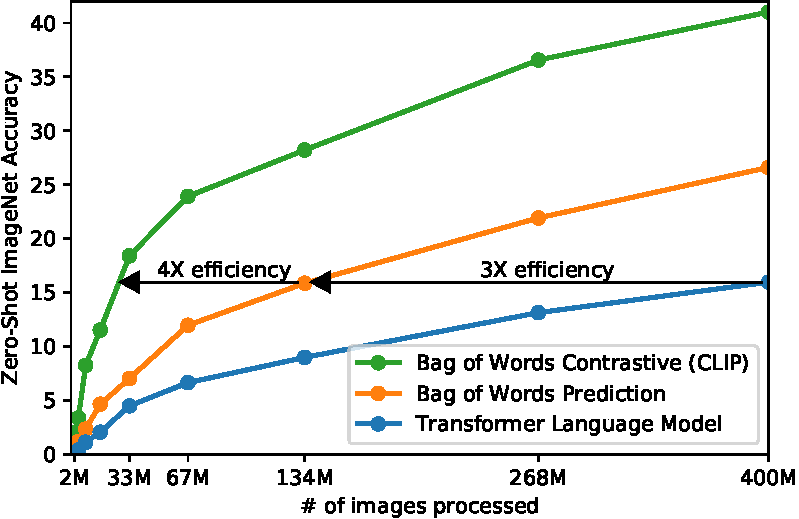
\includegraphics[width=\textwidth]{./images/efficiency-ablation}\framecite{clip}
        \end{column}
    \end{columns}
\end{frame}

\begin{frame}
    \begin{figure}
        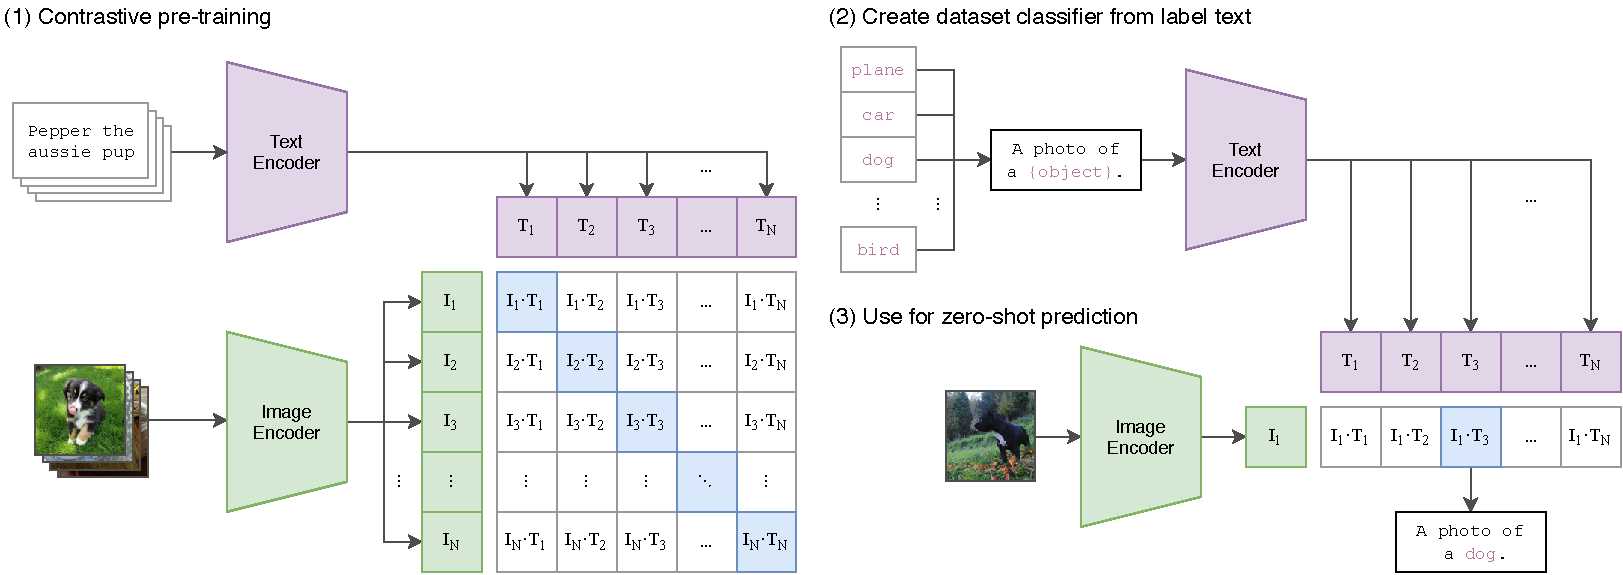
\includegraphics[width=.6\textwidth,trim={0 0 13.5cm 0},clip]{./images/main-diagrams}
        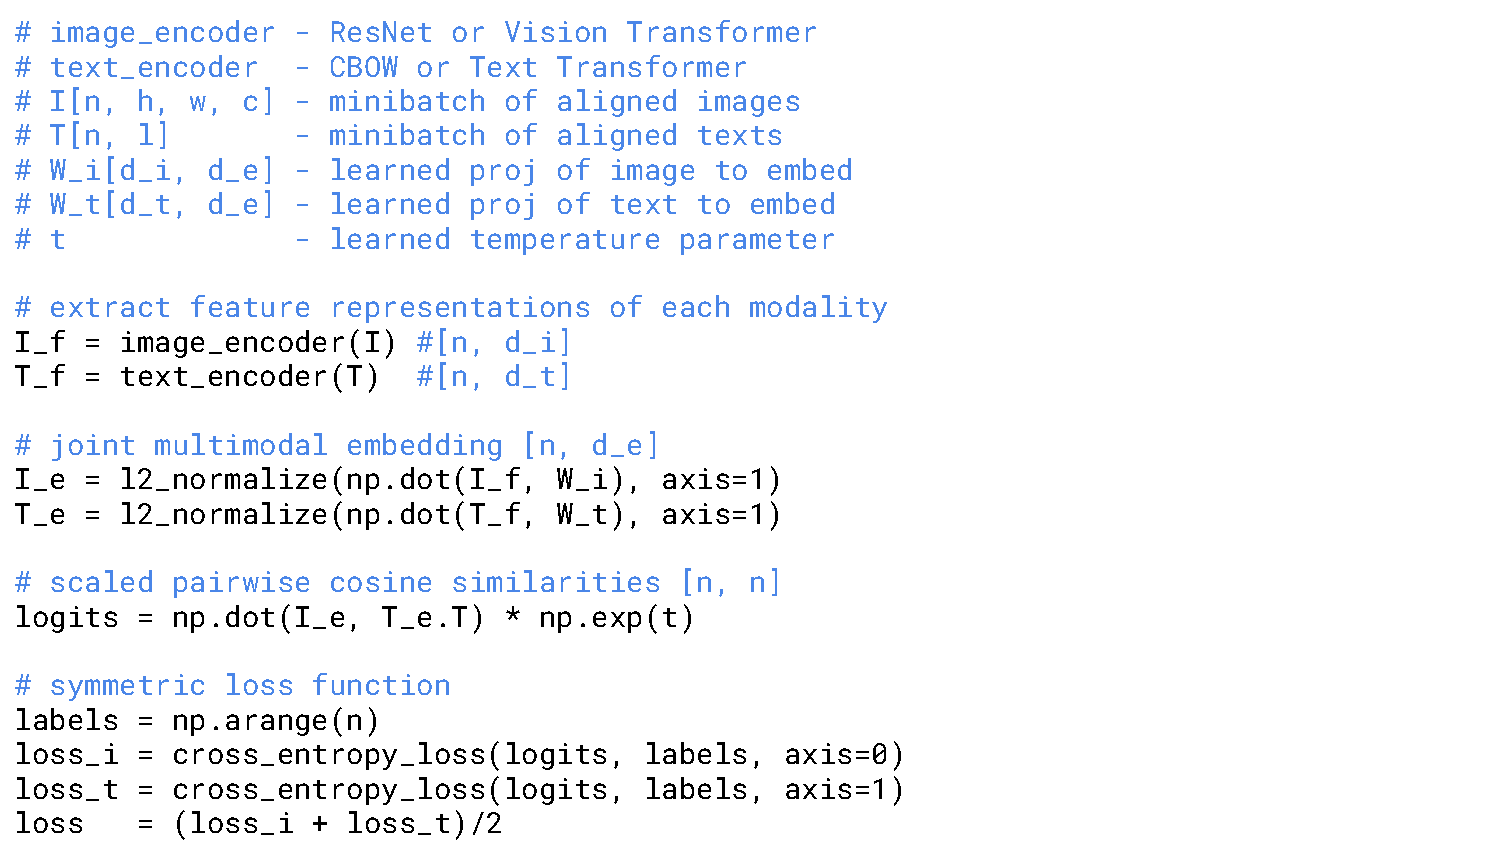
\includegraphics[width=.35\textwidth]{./images/pseudocode}\footfullcite{clip}
    \end{figure}
\end{frame}

\begin{frame}
    \centering
    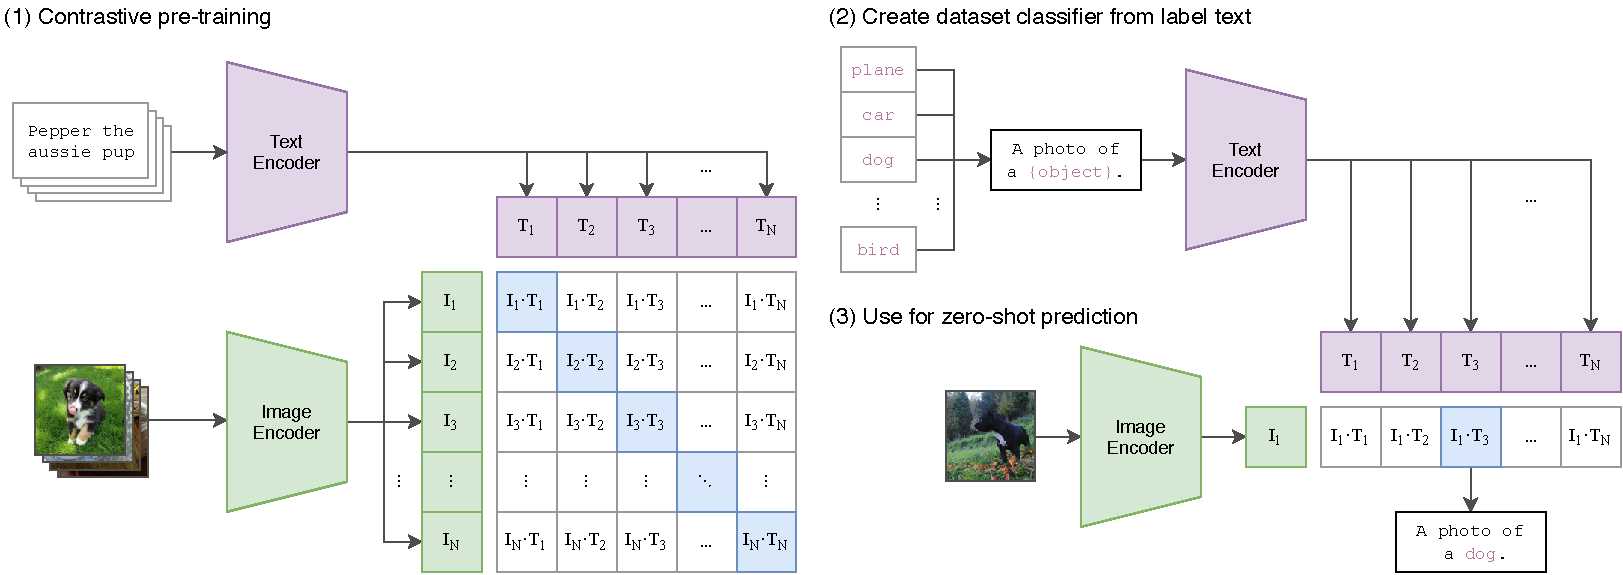
\includegraphics[height=6.5cm,trim={13.5cm 0 0 0},clip]{./images/main-diagrams}\footfullcite{clip}
\end{frame}

% \begin{frame}
%     \frametitle{Underlying Models}
%     \begin{columns}[t]
%         \begin{column}{0.4\textwidth}
%             Text Encoder
%             \begin{itemize}
%                 \item<1-> Transformer
%                 \item<2-> Capacity doesn't affect performance
%             \end{itemize}
%         \end{column}
%         \begin{column}{0.6\textwidth}
%             Image Encoder
%             \begin{itemize}
%                 \item<3-> ResNet with attention layer
%                       \begin{itemize}
%                           \item ResNet-50
%                           \item ResNet-101
%                           \item RN50x4
%                           \item RN50x16
%                           \item<4-> RN50x64: Trained 18 days on 592 V100 GPUs!
%                       \end{itemize}
%                 \item<5-> Vision Transformer
%                       \begin{itemize}
%                           \item ViT-B/16
%                           \item ViT-B/32
%                           \item ViT-L/14: Trained 12 days on 256 V100s
%                           \item<6-> ViT-L/14@336px: Higher resolution,  trained one more epoch. \underline{Performs best!}
%                       \end{itemize}
%             \end{itemize}

%         \end{column}
%     \end{columns}
% \end{frame}

\begin{frame}
    \frametitle{The Dataset}

    \begin{columns}[t]
        \begin{column}{0.5\textwidth}
            Existing datasets
            \begin{itemize}
                \item Crowd-labeled datasets: "only" \~{} 100k images
                \item Large datasets (YFCC100M): Generated filenames, sparse metdata
            \end{itemize}
        \end{column}
        \pause
        \begin{column}{0.5\textwidth}
            Custom dataset: WebImageText (WIT)
            \begin{itemize}
                \item 400 million publicly available image-text pairs
                \item Wide variety: 500.000 different queries, each up to 20.000 image-text pairs
                \item Total word count similar to GPT-2's training data
            \end{itemize}
        \end{column}
    \end{columns}
\end{frame}

\section{Benchmarks}
\begin{frame}
    \frametitle{CLIP vs ResNet-50}
    \begin{columns}[T]
        \begin{column}{0.35\textwidth}
            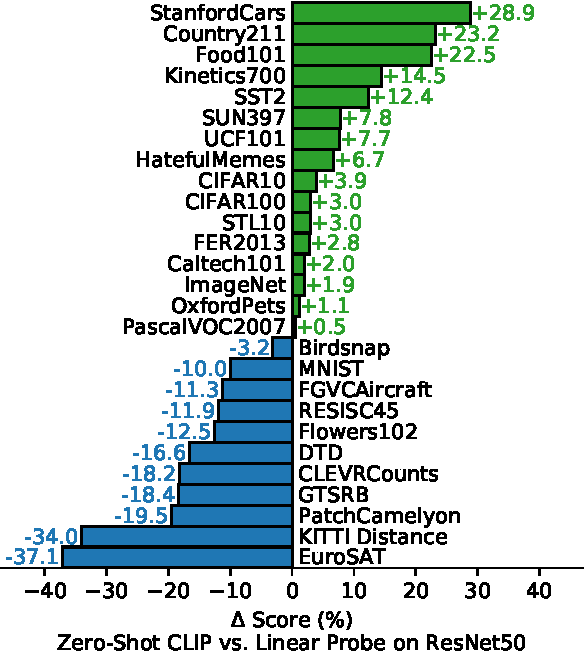
\includegraphics[width=\textwidth]{./images/zs-clip-vs-rn50}\framecite{clip}
        \end{column}
        \pause
        \begin{column}{0.65\textwidth}
            \textbf{Wins}: 16 datasets
            \begin{itemize}
                \item Broad, "general" classes
                \item Datasets with little labeled data
            \end{itemize}

            \pause

            \textbf{Losses}: 11 datasets
            \begin{itemize}
                \item Spezialized classes
                \item Abstract tasks
                \item Counting
                \item Self-driving tasks
            \end{itemize}
        \end{column}
    \end{columns}
\end{frame}

\begin{frame}
    \frametitle{Optimizations}
    \scriptsize
    \begin{columns}[T]
        \begin{column}{0.65\textwidth}
            \textbf{Prompt engineering}
            \begin{itemize}
                \item Provide context: "A photo of a \{ label \}, a type of \{ class \}"
                \item For OCR: Put quotes around the prompt
                \item For sattelite images: "A sattelite photo of a \{ label \}"
                \item Can be further optimized with Context Optimization \framecite{Zhou2021LearningTP}
            \end{itemize}

            \pause
            \vspace{1em}

            \textbf{Ensembling}
            \begin{itemize}
                \item Average over encodings of multiple similar prompts for the same category
                \item Improve performance by 3.5\%
            \end{itemize}
            \vspace{1em}

            Prompt engineering and ensembling improve performance by 5\%
        \end{column}
        \pause
        \begin{column}{0.35\textwidth}
            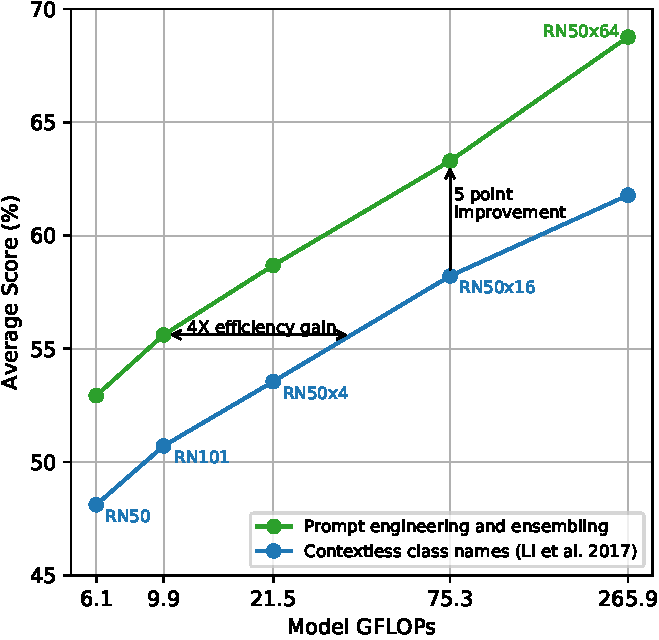
\includegraphics[width=\textwidth]{./images/prompt-engineering}\framecite{clip}
        \end{column}
    \end{columns}
\end{frame}

\section{Conclusion}

\begin{frame}
    \frametitle{Weaknesses}
    \begin{itemize}
        \item<1-> \textbf{Performance}: For many tasks, CLIP is outperformed by specialized models
        \item<2-> \textbf{Prompting}: Sensitive to the input choices, may require prompt engineering to achieve good results
        \item<3-> \textbf{Bias} of the training data is encoded in the model
        \item<4-> \textbf{Dataset} is not publicly available, source is unclear
    \end{itemize}
\end{frame}

\begin{frame}
    \frametitle{Strengths}
    \begin{itemize}
        \item<1-> \textbf{Zero-shot learning}: CLIP can be used for a wide range of tasks without any fine-tuning
        \item<2-> \textbf{Human labor}: No manually labeled data is required
        \item<3-> \textbf{Performance}: CLIP matches or outperforms fine-tuned, specialized models in many tasks
        \item<5-> \textbf{Symmetry}: It's also possible classify a piece of text for a given set of images
        \item<6-> Results are easy to \textbf{reproduce}
    \end{itemize}
\end{frame}

\begin{frame}
    \frametitle{Applications: StyleCLIP}
    Using CLIP to manipulate images with text prompts \footfullcite{patashnik2021styleclip}
    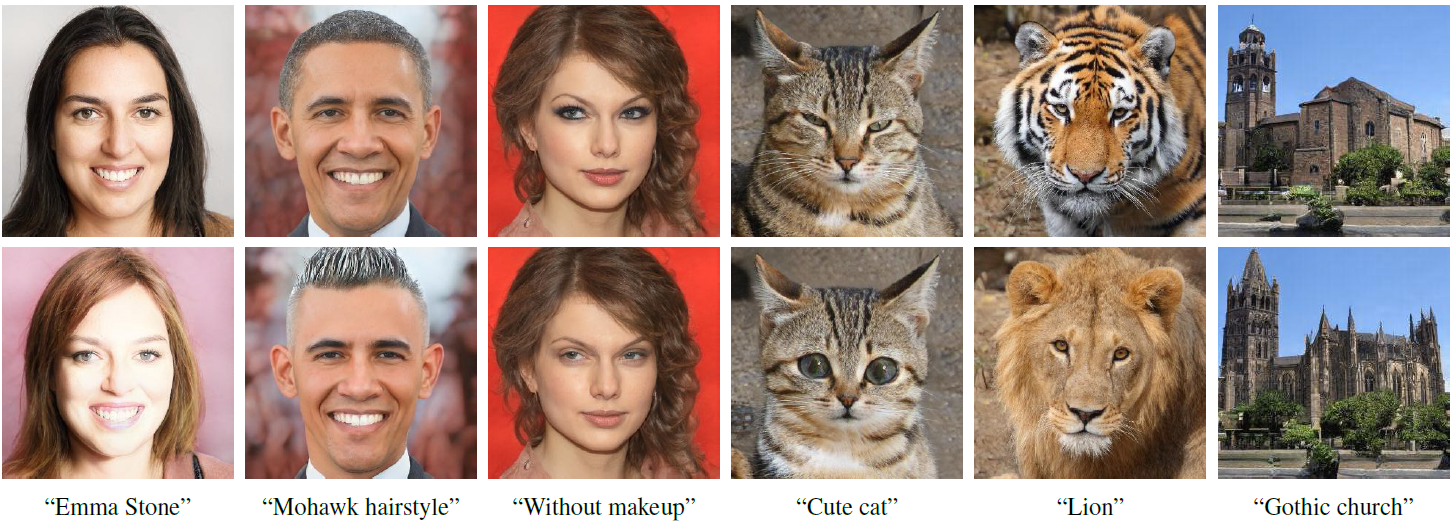
\includegraphics[width=\textwidth]{./images/teaser}
\end{frame}

\begin{frame}
    \frametitle{Applications: Client-side image search}
    Leverage symmetric nature of CLIP to sort/search for images using text prompts \footfullcite{clientsideimagesearch}
    \includegraphics[width=8cm]{./images/image-search}
\end{frame}

\begin{frame}
    \frametitle{Applications: Image generation}
    Use CLIP to generate images from text prompts \footfullcite{ramesh2022hierarchicaltextconditionalimagegeneration}
    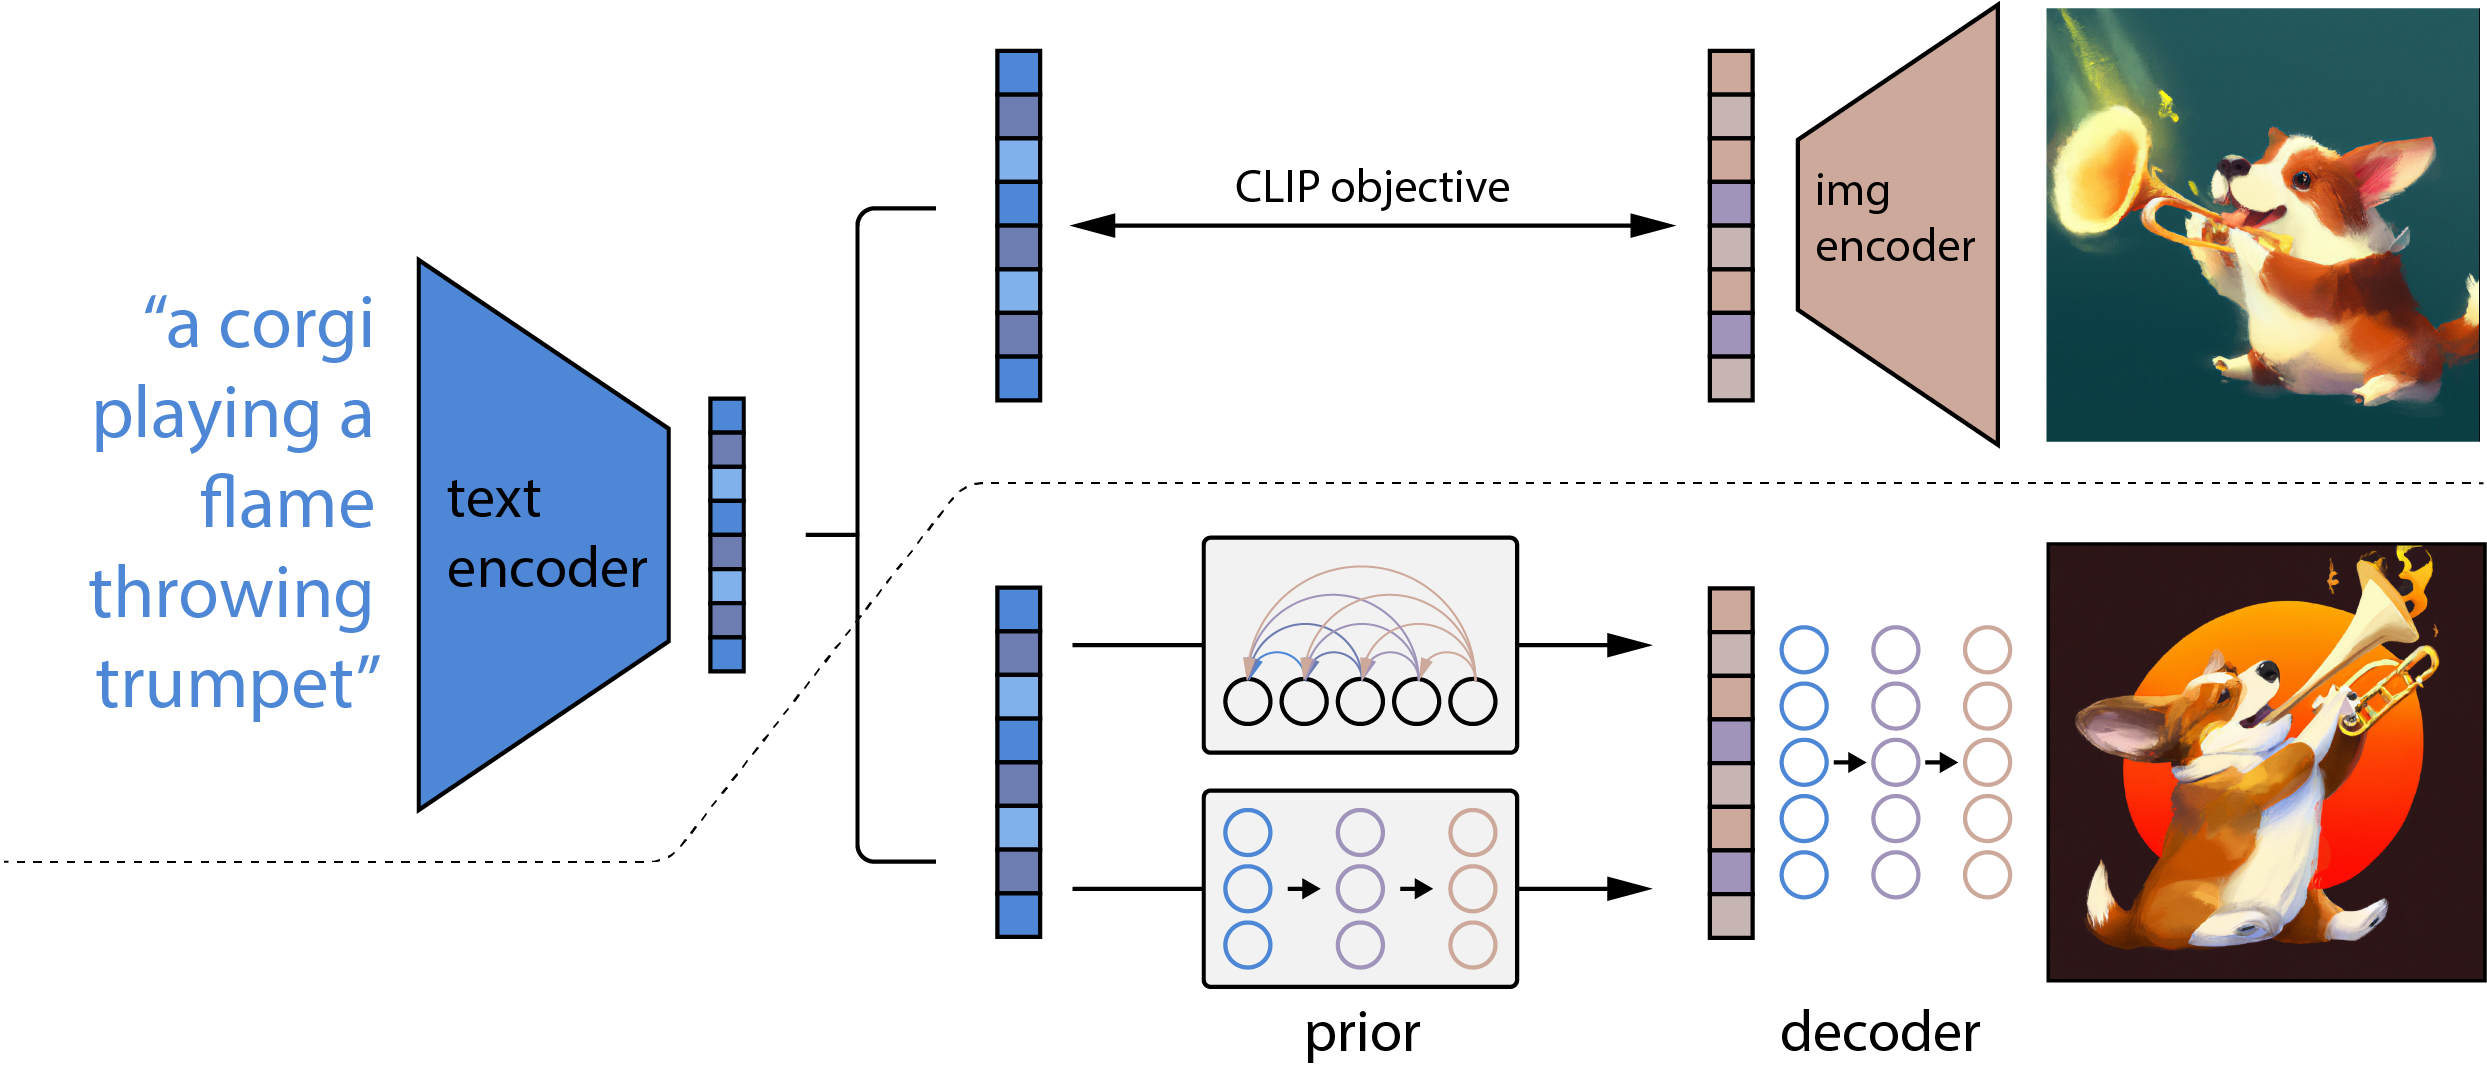
\includegraphics[width=12cm]{./images/unclip-figurehead}
\end{frame}


\begin{frame}[allowframebreaks]
    \frametitle{References}
    \printbibliography
    \LaTeX{}-Beamer template by \href{
\end{frame}

\begin{frame}
    \centering
    \Large If time permits: \par
    \Huge Demo?
\end{frame}

\end{document}
